\documentclass{article}
\usepackage[utf8]{inputenc}
\usepackage{url}
\usepackage{graphicx}
\usepackage{subfigure}
\usepackage{todonotes}
\title{Inpainting d'images}
\date{February 2018}

\begin{document}

\maketitle


\section*{Contexte}


Le contexte du projet est celui de l'\emph{inpainting} d'images  (illustré
dans la figure \ref{fig:my_label}) : étant données une image en entrée
et des parties manquantes (représentées par un masque), il s'agit de
reconstruire les parties manquantes de la manière la plus \emph{plausible}
possible par rapport à la donnée existante dans l'image source.

\begin{figure}[!h]
\centering
\subfigure[]{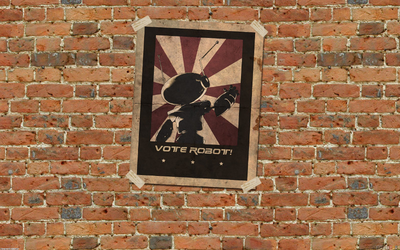
\includegraphics[width=3cm]{wall-robot-400}}
\subfigure[]{
\includegraphics[width=3cm]{wall-robot-400-mask}}
\subfigure[]{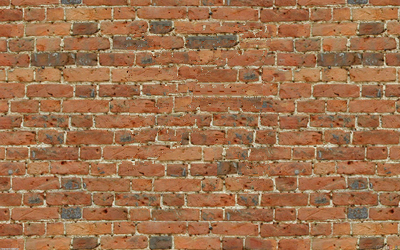
\includegraphics[width=3cm]{out-wall-robot-400}}\\
\subfigure[]{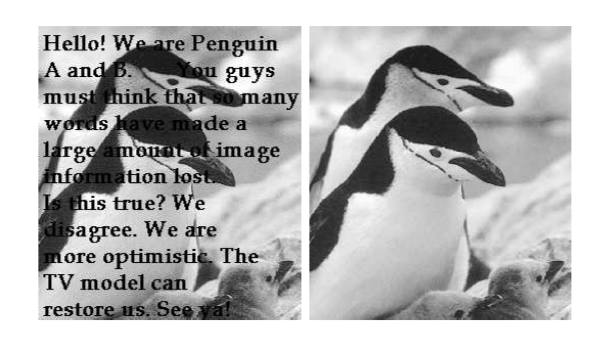
\includegraphics[width=6cm]{peng}}
\caption{Illustration du problème d'inpainting.}
\label{fig:my_label}
\end{figure}
\section*{Objectif}


Dans la littérature, de très nombreuses solutions existent
(variationnelles, basées ``patchs'', réseaux de
neurones...). L'objectif du projet que vous implémentiez une de ces
solutions (ou une solution originale) et que vous en fassiez
l'analyse. Pour cela, nous mettons à votre disposition une série de
publications sur le sujet : survey un peu ancien, mais intéressant
\cite{bertalmio2014inpainting} et par exemple
\cite{masnou1998level,criminisi2003object,barnes2009patchmatch,2017arXiv171203111L}.
Le sujet est extrêmement large et de nombreuses vidéos explicatives
sont disponibles sur internet. N'hésitez pas à interagir avec nous
pour vous aider sur le choix de votre approche. Aucune n'apporte une
réponse ultime au problème, toutes ont des avantages et inconvénients
qu'il vous convient d'analyser.

Nous attendons donc de vous~:
\begin{itemize}
\item Un code d'inpainting prenant en entrée une image et un masque et
  qui complète les pixels manquants du masque (cf Fig
  \ref{fig:my_label}).
\item Un rapport (4 pages max) justifiant vos choix d'implémentation,
  présentant une évaluation expérimentale (qualité, vitesse...) et discutant des
  avantages/limitations de votre approche.
\end{itemize}


Au delà de ces attendus, n'hésitez pas à sortir
du cadre (extensions image shuffling, extensions 3D,
extensions vidéo..).

\section*{Détails}


Par binôme nous attendons une archive avec un répertoire (au nom du
binôme) contenant le code source, un \texttt{Makefile} ou
\texttt{CMakeLists.txt}, un \texttt{readme} pour les indications de
compilation et un rapport (pdf).
\\
\\
\noindent\textbf{Deadline: 23 avril}

\bibliographystyle{alpha}
\bibliography{biblio}
\end{document}
